% !TEX root = ../main.tex
\chapter{Diagnosis Algorithm} \label{ch:diagnosis}
In this chapter will be outlined the diagnosis algorithm\cite{semantic_diagnoser} developed by IBM Research with the collaboration of Michael Maghella, a fellow student at Università degli Studi di Brescia. This algorithm is based on a novel reputation-based approach that makes use of the informations available in the semantic graph to identify cause-effect relationships and use these relationships to isolate relevant causes basing the diagnosis on the timeseries data.
\section{General description}
The diagnosis activity is comprised of three main step:
\begin{itemize}
  \item fault detection, that is the discovery of the fault. A diagnoser needs to be able to tell apart the normal behaviours from faulty ones. This is done, in this approach, through the rules discovered while learning the normal behaviour of a building (see \autoref{subsec:learn_behaviour}). Whenever a fault is detected the diagnosis process ought to start.
  \item fault isolation, that is the discovery of the causes of the fault. It is a key step for enabling a precise diagnosis of the problem. In this approach informations derived from the semantic graph are used to narrow down the set of possible faults to the most relevant ones.
  \item fault identification, that is to determine with some confidence which are the actual causes of a fault among all the possible causes. The proposed diagnoser implements a voting scheme to identify these causes.
\end{itemize}
While explaining the diagnosis approach, it will be used the same model presented in \autoref{ch:model} ( \autoref{fig:ex_building_full}), that will be represented in a compact notation shown in \autoref{fig:simple_model}, where every component is an instance of a concept with the same name (internalized representation).
\begin{figure}
  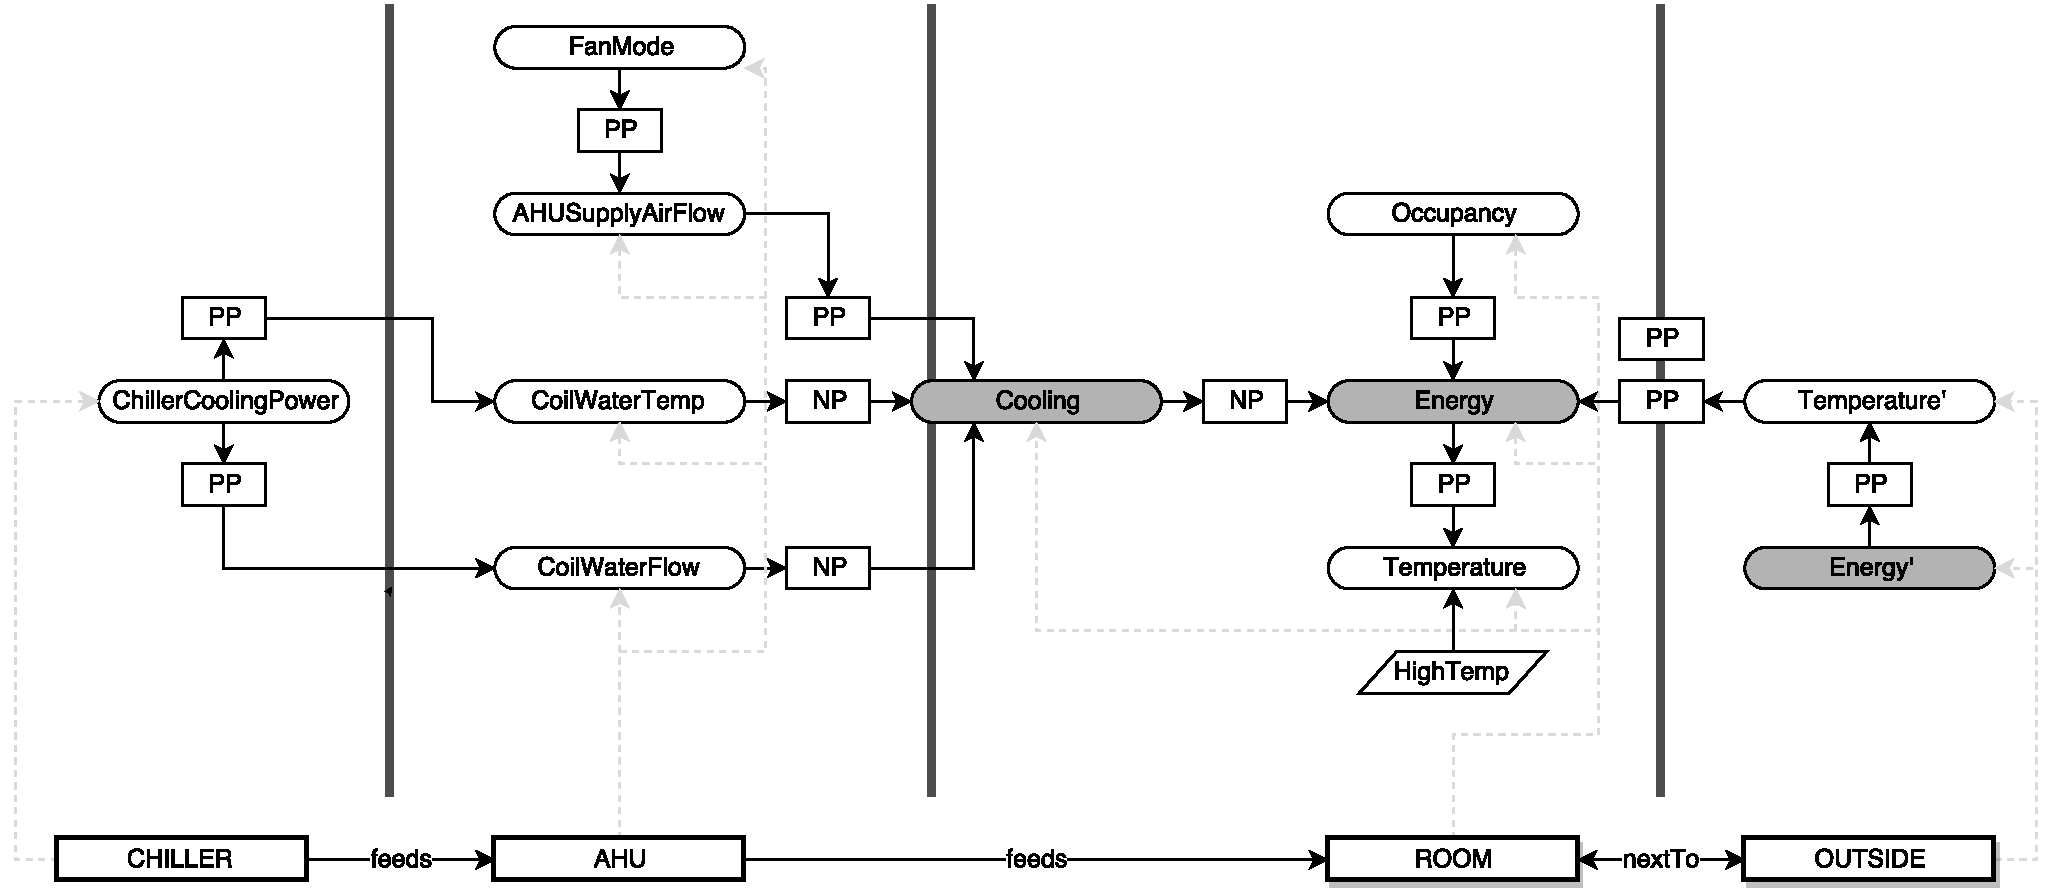
\includegraphics[width=\textwidth]{simple_diagnosis_ex.pdf}
  \caption{Internalized model of the example building}
  \label{fig:simple_model}
\end{figure}
The diagnoser is run every time an anomaly is detected in the timeseries. An anomaly is intended as a deviation from the normal behaviour clearly detectable by some preset upper and lower bounds, therefore an anomaly can be classified as high or low.
It is assumed that an anomaly is symptom of some kind of fault in the system. The algorithm starts, as soon as the anomaly is detected, by identifying the semantic type of the anomaly and the potential causes in the graph. It proceeds computing the voting vector and, eventually, it is recursively executed for all those properties that get a voting score equals or greater then one. When no other causes with a high score are left, the algorithm terminates and produces a list of the detected causes along with the name of the faulty properties, the semantic type of the faults and the estimatation, expressed in percentage, of the responsability of those causes towards the diagnosed anomaly.
\begin{algorithm}
  \caption{General diagnosis algorithm}\label{diagnosis}
  \begin{algorithmic}[1]
    \Require
      \Statex the anomaly $A$,
      \Statex the semantic graph $\mathcal{G}$
    \Ensure a set $C_A$ of possible causes of the anomaly
    \Procedure{diagnoseAnomaly}{$A,\mathcal{G}$}
    \State $T\leftarrow$ \Call{getSemanticTypeOfAnomaly}{$A$}
    \State $PC_A\leftarrow$ \Call{getPossibleCausesInGraph}{$A,T,\mathcal{G}$}
    \State $C_A\leftarrow\emptyset$
    \State $\bm v\leftarrow$ \Call{computeReputationVoteVector}{$A,T,PC_A$}
    \ForAll {$p\in PC_A$}
    \If{$\bm v[p]\geq 1$}
    \State $C_p\leftarrow$ \Call{diagnoseAnomaly}{$p,\mathcal{G}$} \Comment{diagnose subtree}
    \If{$C_p\neq\emptyset$}
    \State $C_A\leftarrow C_A\cup C_p$
    \Else
    \State $C_A\leftarrow C_A\cup\{p\}$ \Comment{$p$ is a root cause}
    \EndIf
    \EndIf
    \EndFor
    \EndProcedure
  \end{algorithmic}
\end{algorithm}
\paragraph{Potential causes}
The first non-trivial operation of the algorithm is the identification of the possible causes of a given an anomaly. A potential cause is an observation made by a sensor that observe a property and such that the following hold:
\begin{enumerate}
  \item the property observed by the sensor is an input of a process that directly output to the anomaly, or it is connected to the anomalous property by a chain of unobservable properties
  \item it is observable.
\end{enumerate}
The properties and their relationships with the anomaly are all encoded in the semantic graph and are therefore accessible via reasoning. The approach is also interested in the semantic type of the anomaly and of the possible causes.
Retrieveing the possible causes of an anomaly is possible because in the graph, anomalies are observations made by a sensor that measures a property.
\begin{figure}
  \begin{subfigure}[b]{\textwidth}
    \centering
      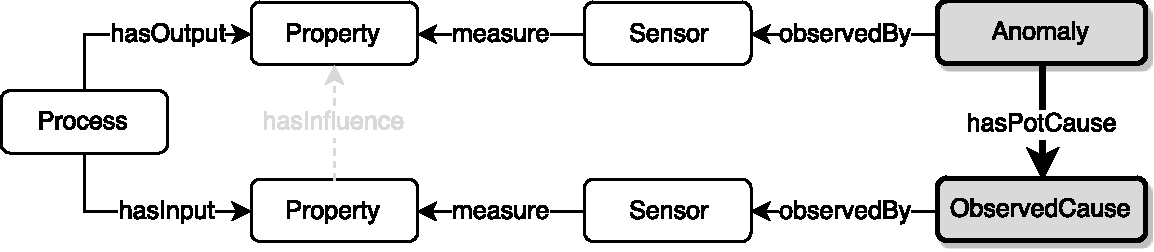
\includegraphics[width=1\linewidth]{direct_cause.pdf}
      \caption{Direct influence}
      \label{fig:direct_influence}
  \end{subfigure}
  \begin{subfigure}[b]{\textwidth}
    \centering
      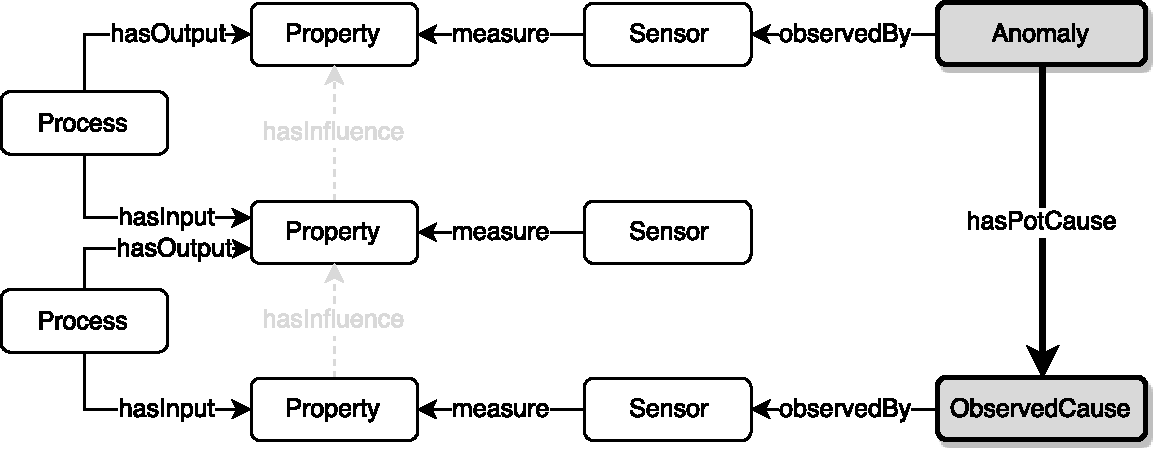
\includegraphics[width=1\linewidth]{unobs_chain.pdf}
      \caption{Chain of unobservables properties}
      \label{fig:chain_unobs}
  \end{subfigure}
  \caption{Detection of potential causes}
  \label{fig:pot_causes}
\end{figure}
\autoref{fig:pot_causes} shows the possible ways to retrieve a potential cause of a property. In both figures the situation respect the conditions given earlier in the chapter regarding potential causes.
The causes retrieved at this point are the ones that are correlated at various degrees to the anomaly and are the only ones that can help to produce a diagnosis. At this point it is important to preserve the semantic informations about the processes involved since this information is at the base of the voting algorith. When talking about ``semantic informations'' of the process it is meant the replacement of a chain of properties with a single, direct process whose type is infered from the ones of the chain. For example it can be seen in \autoref{fig:chain_composition} that the temperature in a room is influenced by the occupancy property of the room through a chain of a PT1 process and a PP process, both involving the unobservable energy property. This means that the temperature is influenced by the occupancy through a direct PT1 process.
\begin{figure}
  \centering
  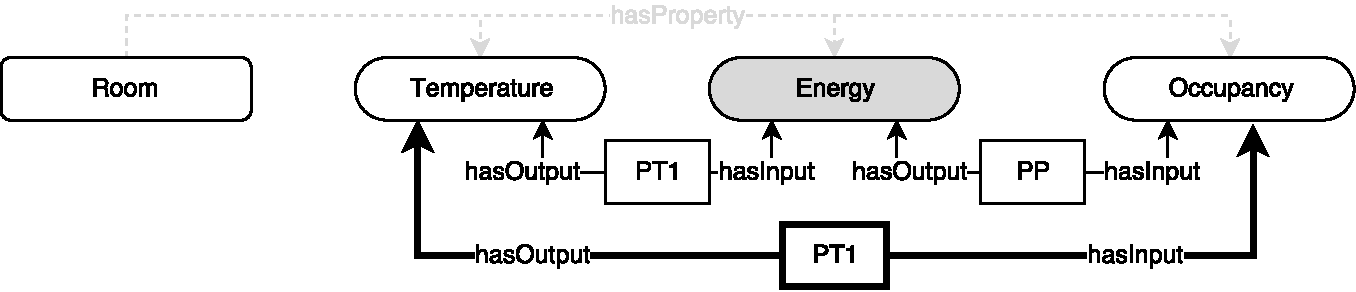
\includegraphics[width=1\textwidth]{process_chaining.pdf}
  \caption{Process chains compositions}
  \label{fig:chain_composition}
\end{figure}
\autoref{tab:process_chains_combination} shows the possible combinations for the most common type of processes usedm that are the positive correlation, the negative correlation and the lag processes.
\begin{table}
  \centering
  \caption{Derived processes from most common process chains}
  \label{tab:process_chains_combination}
  \begin{tabular}{lll}
    \hline\textbf{First process} & \textbf{Second process} & \textbf{Derived process}\\\hline
    Positive correlated & Positive correlated & Positive correlated\\
    Positive correlated & Negative correlated & Negative correlated\\
    Negative correlated & Positive correlated & Negative correlated\\
    Negative correlated & Negative correlated & Positive correlated\\
    Any & Lag & Lag \\\hline
  \end{tabular}
\end{table}
Given these new processes, that directly correlate an anomaly to its potential causes, it is possible to infer the entity of the potential cause. This information is computed thanks to the intuition that the type of process correlating two observation carries qualitative information about the output. It is possible, for example, predict that an observation that is influenced by a positive correlation process whose input is an observation that is high is high itself. The ontology defines the combinations listed in \autoref{fig:anomaly_type_prediction}.
\begin{table}
  \centering
  \caption{Predicted value of an observation based on the process it depends on and the input to such process}
  \label{fig:anomaly_type_prediction}
  \begin{tabular}{lll}
    \hline\textbf{Anomaly type} & \textbf{Process type} & \textbf{Cause type}\\\hline
    High & Positive correlated & High\\
    High & Negative correlated & Low\\
    Low & Positive correlated & High\\
    Low & Negative correlated & Low \\
    Any & Lag & Lag \\\hline
  \end{tabular}
\end{table}
